\documentclass{article}

\usepackage{polski}
\usepackage{amsmath, array}
\usepackage{graphicx}
\usepackage{float}
\usepackage{subfig}
\usepackage{multirow}
\usepackage{enumitem}

\title{Laboratorium 6}
\author{\textbf{Łukasz Wala}\\
    \textit{AGH, Wydział Informatyki, Elektroniki i Telekomunikacji} \\
    \textit{Teoria Współbieżności 2022/23}}
\date{Kraków, \today}

\begin{document}
\maketitle

\section{Treść zadania 1}
Problem czytelników i pisarzy proszę rozwiązać przy pomocy: semaforów i zmiennych warunkowych.

Proszę wykonać pomiary dla różnej ilości czytelkników czytelników (10-100) i pisarzy (od 1 do 10).
W sprawozdaniu proszę narysować 3D wykres czasu w zależności od liczby wątków i go zinterpretować.

\section{Implementacja zadania 1 - semafory}

Zaimplementowana zostanie wersja, gdzie zagłodzony może zostać pisarz, tzn. czytelnik nie musi czekać, 
nawet jeżeli jakiś pisarz już czeka.

\begin{verbatim}
class Writer extends Thread {
    Resource resource;
    int count;

    public Writer(Resource resource, int count) {
        this.resource = resource;
        this.count = count;
    }

    public void run() {
        for (int i=0; i<count; ++i) {
            try {
                resource.write();
            } catch (InterruptedException e) {
                System.exit(1);
            }
        }
    }
}

class Reader extends Thread {
    Resource resource;
    int count;

    public Reader(Resource resource, int count) {
        this.resource = resource;
        this.count = count;
    }

    public void run() {
        for (int i=0; i<count; ++i) {
            try {
                resource.read();
            } catch (InterruptedException e) {
                System.exit(1);
            }
        }
    }
}

class Resource {
    Semaphore resource = new Semaphore(1);
    Semaphore mutex = new Semaphore(1);
    int readCount = 0;

    public void write() throws InterruptedException {
        resource.acquire();

        // writing
        Thread.sleep(ThreadLocalRandom.current().nextInt(10) * 9);

        resource.release();
    }

    public void read() throws InterruptedException {
        mutex.acquire();
        ++readCount;
        if (readCount == 1) resource.acquire();
        mutex.release();

        // reading
        Thread.sleep(ThreadLocalRandom.current().nextInt(10) * 3);

        mutex.acquire();
        --readCount;
        if (readCount == 0) resource.release();
        mutex.release();
    }
}

public class ReadersWriters {
    public static void main(String[] args) throws InterruptedException {
        for (int writers=1; writers<11; ++writers) {
            for (int readers=10; readers<101; readers += 10) {
                Resource resource = new Resource();
            
                ExecutorService service = Executors.newFixedThreadPool(writers + readers);

                long startTime = System.nanoTime();

                for (int i=0; i<writers; ++i) {
                    service.submit(new Writer(resource, 3));
                }

                for (int i=0; i<readers; ++i) {
                    service.submit(new Reader(resource, 3));
                }

                service.shutdown();
                while (!service.awaitTermination(24L, TimeUnit.HOURS)) 
                    ;

                long endTime = System.nanoTime();


                System.out.print(writers + " " + readers + " ");
                System.out.println((endTime - startTime)/1000000);
            }
        }
    }
}
\end{verbatim}

Poniżej znajduje się wykres zależności czasu od liczby pisarzy od liczby czytelników, gdzie każdy czytelnik
i pisarz wykonują 3 iteracje pisania/czytania po czym się wyłączają:

\begin{figure}[H]
    \centering
    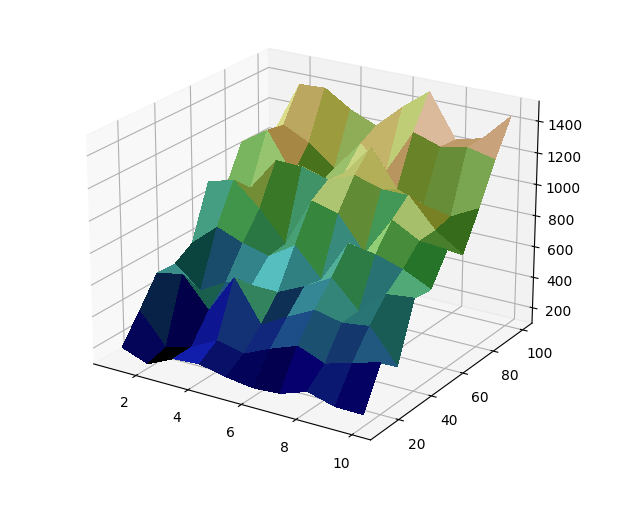
\includegraphics[width=\textwidth]{figure_1.png}
    \caption{Wykres dla implementacji z semaforami (ms)}
\end{figure}

\section{Implementacja zadania 1 - zmienne warunkowe}

Zmiana w tym rozwiązaniu następuje tylko w klasie \textit{Resource}:

\begin{verbatim}
class Resource {
    ReentrantLock lock = new ReentrantLock();
    Condition isAvailableCondition = lock.newCondition();
    boolean isAvailable = true;
    int readCount = 0;

    public void write() throws InterruptedException {
        lock.lock();
        while (!isAvailable) {
            isAvailableCondition.await();
        }
        isAvailable = false;
        lock.unlock();

        // writing
        Thread.sleep(ThreadLocalRandom.current().nextInt(10) * 9);

        lock.lock();
        isAvailable = true;
        isAvailableCondition.signalAll();
        lock.unlock();
    }

    public void read() throws InterruptedException {
        lock.lock();
        ++readCount;
        if (readCount == 1) {
            while (!isAvailable) {
                isAvailableCondition.await();
            }
            isAvailable = false;
        }
        lock.unlock();

        // reading
        Thread.sleep(ThreadLocalRandom.current().nextInt(10) * 3);

        lock.lock();
        --readCount;
        if (readCount == 0) isAvailable = true;
        isAvailableCondition.signalAll();
        lock.unlock();
    }
}
\end{verbatim}

Poniżej wykres:

\begin{figure}[H]
    \centering
    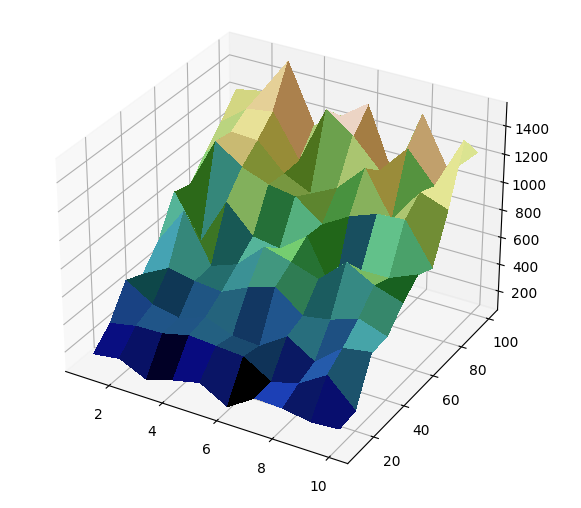
\includegraphics[width=\textwidth]{figure_2.png}
    \caption{Wykres dla implementacji z \textit{lock} (ms)}
\end{figure}

W przypadki obu wykresów można łatwo zauważyć, że wraz ze wzrostem liczby czytelników rośnie czas 
działania programu (fizyczne ograniczenia maszyny sprawiają, że prawdziwie równolegle wykonywana
jest jedynie część wątków czytelników, nawet jeżeli zasady problemu pozwalałyby na to, żeby wszystkie
były wykonywane jednocześnie). Wzrost liczby pisarzy ma mniejszy wpływ na czas działania, jednak ich
liczba jest inkrementowana o mniejszą wartość.

\section{Treść zadania 2}

\begin{enumerate}
    \item 
    Proszę zaimplementować listę, w której każdy węzeł składa się z wartości typu \textit{Object}, 
    referencji do następnego węzła oraz zamka (\textit{lock}).
    \item
    Proszę zastosować metodę drobnoziarnistego blokowania do następujących metod listy:
    \begin{verbatim}
    boolean contains(Object o);  // czy lista zawiera element o
    boolean remove(Object o);  // usuwa pierwsze wystąpienie elementu o
    boolean add(Object o);  // dodaje element o na końcu listy  
    \end{verbatim}
    \item
    Proszę porównać wydajność tego rozwiązania w stosunku do listy z jednym zamkiem 
    blokującym dostęp do całości. Należy założyć, że koszt czasowy operacji na elemencie 
    listy (porównanie, wstawianie obiektu) może być duży - proszę wykonać pomiary dla różnych 
    wartości tego kosztu.
\end{enumerate}




\section{Implementacja zadania 2}

Poniżej implementacja listy spełniającej warunki zadania:

\begin{verbatim}
class FineGrainedList {
    public class ListElement {
        public ReentrantLock lock = new ReentrantLock();
        public Object value;
        public ListElement next;

        public ListElement(Object value, ListElement next) {
            this.value = value;
            this.next = next;
        }
    }

    // dummy first element
    ListElement first = new ListElement(null, null);

    private boolean sublistContains(Object value, ListElement element) {
        if (element.value == value) {
            element.lock.unlock();
            return true;
        }
        if (element.next != null) {
            element.next.lock.lock();
            element.lock.unlock();
            return sublistContains(value, element.next);
        }
        element.lock.unlock();
        return false;
    }

    public boolean contains(Object value) {
        first.lock.lock();
        if (first.next == null) {
            first.lock.unlock();
            return false;
        }
        return sublistContains(value, first.next);
    }

    private void sublistRemove(Object value, ListElement element, ListElement prevElement) {
        if (element.value == value) {
            prevElement.next = element.next;
            prevElement.lock.unlock();
            element.lock.unlock();
        } else if (element.next != null) {
            prevElement.lock.unlock();
            element.next.lock.lock();
            sublistRemove(value, element.next, element);
        } else {
            prevElement.lock.unlock();
            element.lock.unlock();
        }
    }

    public void remove(Object value) {
        if (first.next != null) {
            first.lock.lock();
            first.next.lock.lock();
            sublistRemove(value, first.next, first);
        }
    }

    private void sublistAdd(Object value, ListElement element) {
        if (element.next == null) {
            element.next = new ListElement(value, null);
            element.lock.unlock();
        } else {
            element.next.lock.lock();
            element.lock.unlock();
            sublistAdd(value, element.next);
        }
    }
    
    public void add(Object value) {
        first.lock.lock();
        sublistAdd(value, first);
    }
}
\end{verbatim}

Teraz nastąpi porównanie wydajności, ale do tego potrzebna jest jeszcze implementacja listy z jednym
zamkiem:

\begin{verbatim}
class BlockingList {
    public class ListElement {
        public Object value;
        public ListElement next;

        public ListElement(Object value, ListElement next) {
            this.value = value;
            this.next = next;
        }
    }

    ReentrantLock lock = new ReentrantLock();

    // dummy first element
    ListElement first = new ListElement(null, null);

    private boolean sublistContains(Object value, ListElement element) {
        if (element.value == value) return true;
        else if (element.next != null) return sublistContains(value, element.next);
        else return false;
    }

    public boolean contains(Object value) {
        lock.lock();
        if (first.next == null) return false;
        boolean res = sublistContains(value, first.next);
        lock.unlock();
        return res;
    }

    private void sublistRemove(Object value, ListElement element, ListElement prevElement) {
        if (element.value == value) {
            prevElement.next = element.next;
        } else if (element.next != null) {
            sublistRemove(value, element.next, element);
        }
    }

    public void remove(Object value) {
        lock.lock();
        if (first.next != null) {
            sublistRemove(value, first.next, first);
        }
        lock.unlock();
    }

    private void sublistAdd(Object value, ListElement element) {
        if (element.next == null) element.next = new ListElement(value, null);
        else sublistAdd(value, element.next);
    }

    public void add(Object value) {
        lock.lock();
        sublistAdd(value, first);
        lock.unlock();
    }
}
\end{verbatim}

Jak można było przypuszczać, lista z blokowaniem drobnoziarnistym działa znacznie efektywniej, gdy
jest używana równolegle przez wiele wątków, ponieważ nie musi blokować elementów, które i tak nie są
przetważane. W momencie, gdy np. jeden wątke chce wstawić element na końcu listy, musi przeiterować 
po wszystkich innych elementach. W przypadku listy z blokowaniem drobnoziarnistym (przy założeniu, że interowanie
jest szybkie, a wstawianie czasochłonne) inne wątki mogą prawie natychmiast operować na wszystkich elementach
listy z wyjątkiem ostatniego, w przypadku zwyczajnej listy blokującej, pozostałe wątki muszą czekać, aż
element nie zostanie wstawiony na koniec.

\section{Wnioski}

W zależności od problemu, trzeba brać pod uwagę, czy, pomimo że operacje są wykonywanie bezpiecznie z
perspektywy dostępu do zasobów, któraś grupa wątków działająca na zasobie nie zostanie zagłodzona (
w problemie czytelników i pisarzy łatwo sprawić, że pomimo pozornie poprawnego dostępu do zasobu,
albo pisarze albo czytelnicy mogą nigdy nie doczekać się swojej kolei na dostęp do niego).

Ważnym aspektem programowania równogległego jest, oprócz zapewnienia bezpieczeństwa dostępu do zasobu,
sprawienie, żeby zasoby niewykorzystywane w danym momencie czasu nie były niepotrzebnie blokowane.
W przypadku operacji na listach nie ma sensu blokowanie całej listy, lepiej blokować indywidualne elementy,
co znacznie przyśpiesza niektóre operacje.

\section{Bibliografia}

\begin{enumerate}
    \item 
    Dokumentacja języka Java - docs.oracle.com
\end{enumerate}

\end{document}